\documentclass[tikz,border=10pt]{standalone}
\usetikzlibrary{shapes.geometric, arrows, graphs, arrows.meta,decorations.pathmorphing,backgrounds,positioning,fit,petri}

\begin{document}

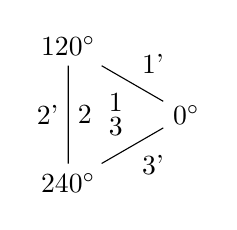
\begin{tikzpicture}[auto]
  \node (a) at (0:1) {$0^\circ$};
  \node (b) at (120:1) {$120^\circ$};
  \node (c) at (240:1) {$240^\circ$};

  \draw (a) to node {1} node [swap] {1'} (b)
        (b) to node {2} node [swap] {2'} (c)
        (c) to node {3} node [swap] {3'} (a);
\end{tikzpicture}

\end{document}

